
% Default to the notebook output style

    


% Inherit from the specified cell style.




    
\documentclass{article}

    
    
    \usepackage{graphicx} % Used to insert images
    \usepackage{adjustbox} % Used to constrain images to a maximum size 
    \usepackage{color} % Allow colors to be defined
    \usepackage{enumerate} % Needed for markdown enumerations to work
    \usepackage{geometry} % Used to adjust the document margins
    \usepackage{amsmath} % Equations
    \usepackage{amssymb} % Equations
    \usepackage{eurosym} % defines \euro
    \usepackage[mathletters]{ucs} % Extended unicode (utf-8) support
    \usepackage[utf8x]{inputenc} % Allow utf-8 characters in the tex document
    \usepackage{fancyvrb} % verbatim replacement that allows latex
    \usepackage{grffile} % extends the file name processing of package graphics 
                         % to support a larger range 
    % The hyperref package gives us a pdf with properly built
    % internal navigation ('pdf bookmarks' for the table of contents,
    % internal cross-reference links, web links for URLs, etc.)
    \usepackage{hyperref}
    \usepackage{longtable} % longtable support required by pandoc >1.10
    \usepackage{booktabs}  % table support for pandoc > 1.12.2
    \usepackage{indentfirst}

    
    
    \definecolor{orange}{cmyk}{0,0.4,0.8,0.2}
    \definecolor{darkorange}{rgb}{.71,0.21,0.01}
    \definecolor{darkgreen}{rgb}{.12,.54,.11}
    \definecolor{myteal}{rgb}{.26, .44, .56}
    \definecolor{gray}{gray}{0.45}
    \definecolor{lightgray}{gray}{.95}
    \definecolor{mediumgray}{gray}{.8}
    \definecolor{inputbackground}{rgb}{.95, .95, .85}
    \definecolor{outputbackground}{rgb}{.95, .95, .95}
    \definecolor{traceback}{rgb}{1, .95, .95}
    % ansi colors
    \definecolor{red}{rgb}{.6,0,0}
    \definecolor{green}{rgb}{0,.65,0}
    \definecolor{brown}{rgb}{0.6,0.6,0}
    \definecolor{blue}{rgb}{0,.145,.698}
    \definecolor{purple}{rgb}{.698,.145,.698}
    \definecolor{cyan}{rgb}{0,.698,.698}
    \definecolor{lightgray}{gray}{0.5}
    
    % bright ansi colors
    \definecolor{darkgray}{gray}{0.25}
    \definecolor{lightred}{rgb}{1.0,0.39,0.28}
    \definecolor{lightgreen}{rgb}{0.48,0.99,0.0}
    \definecolor{lightblue}{rgb}{0.53,0.81,0.92}
    \definecolor{lightpurple}{rgb}{0.87,0.63,0.87}
    \definecolor{lightcyan}{rgb}{0.5,1.0,0.83}
    
    % commands and environments needed by pandoc snippets
    % extracted from the output of `pandoc -s`
    \providecommand{\tightlist}{%
      \setlength{\itemsep}{0pt}\setlength{\parskip}{0pt}}
    \DefineVerbatimEnvironment{Highlighting}{Verbatim}{commandchars=\\\{\}}
    % Add ',fontsize=\small' for more characters per line
    \newenvironment{Shaded}{}{}
    \newcommand{\KeywordTok}[1]{\textcolor[rgb]{0.00,0.44,0.13}{\textbf{{#1}}}}
    \newcommand{\DataTypeTok}[1]{\textcolor[rgb]{0.56,0.13,0.00}{{#1}}}
    \newcommand{\DecValTok}[1]{\textcolor[rgb]{0.25,0.63,0.44}{{#1}}}
    \newcommand{\BaseNTok}[1]{\textcolor[rgb]{0.25,0.63,0.44}{{#1}}}
    \newcommand{\FloatTok}[1]{\textcolor[rgb]{0.25,0.63,0.44}{{#1}}}
    \newcommand{\CharTok}[1]{\textcolor[rgb]{0.25,0.44,0.63}{{#1}}}
    \newcommand{\StringTok}[1]{\textcolor[rgb]{0.25,0.44,0.63}{{#1}}}
    \newcommand{\CommentTok}[1]{\textcolor[rgb]{0.38,0.63,0.69}{\textit{{#1}}}}
    \newcommand{\OtherTok}[1]{\textcolor[rgb]{0.00,0.44,0.13}{{#1}}}
    \newcommand{\AlertTok}[1]{\textcolor[rgb]{1.00,0.00,0.00}{\textbf{{#1}}}}
    \newcommand{\FunctionTok}[1]{\textcolor[rgb]{0.02,0.16,0.49}{{#1}}}
    \newcommand{\RegionMarkerTok}[1]{{#1}}
    \newcommand{\ErrorTok}[1]{\textcolor[rgb]{1.00,0.00,0.00}{\textbf{{#1}}}}
    \newcommand{\NormalTok}[1]{{#1}}
    
    % Define a nice break command that doesn't care if a line doesn't already
    % exist.
    \def\br{\hspace*{\fill} \\* }
    % Math Jax compatability definitions
    \def\gt{>}
    \def\lt{<}
    % Document parameters
    \title{Homework 9}
    \author{Roly Vicar\'ia \\ STAT500 Summer 2015}
    
    
    

    % Pygments definitions
    
\makeatletter
\def\PY@reset{\let\PY@it=\relax \let\PY@bf=\relax%
    \let\PY@ul=\relax \let\PY@tc=\relax%
    \let\PY@bc=\relax \let\PY@ff=\relax}
\def\PY@tok#1{\csname PY@tok@#1\endcsname}
\def\PY@toks#1+{\ifx\relax#1\empty\else%
    \PY@tok{#1}\expandafter\PY@toks\fi}
\def\PY@do#1{\PY@bc{\PY@tc{\PY@ul{%
    \PY@it{\PY@bf{\PY@ff{#1}}}}}}}
\def\PY#1#2{\PY@reset\PY@toks#1+\relax+\PY@do{#2}}

\expandafter\def\csname PY@tok@gd\endcsname{\def\PY@tc##1{\textcolor[rgb]{0.63,0.00,0.00}{##1}}}
\expandafter\def\csname PY@tok@gu\endcsname{\let\PY@bf=\textbf\def\PY@tc##1{\textcolor[rgb]{0.50,0.00,0.50}{##1}}}
\expandafter\def\csname PY@tok@gt\endcsname{\def\PY@tc##1{\textcolor[rgb]{0.00,0.27,0.87}{##1}}}
\expandafter\def\csname PY@tok@gs\endcsname{\let\PY@bf=\textbf}
\expandafter\def\csname PY@tok@gr\endcsname{\def\PY@tc##1{\textcolor[rgb]{1.00,0.00,0.00}{##1}}}
\expandafter\def\csname PY@tok@cm\endcsname{\let\PY@it=\textit\def\PY@tc##1{\textcolor[rgb]{0.25,0.50,0.50}{##1}}}
\expandafter\def\csname PY@tok@vg\endcsname{\def\PY@tc##1{\textcolor[rgb]{0.10,0.09,0.49}{##1}}}
\expandafter\def\csname PY@tok@m\endcsname{\def\PY@tc##1{\textcolor[rgb]{0.40,0.40,0.40}{##1}}}
\expandafter\def\csname PY@tok@mh\endcsname{\def\PY@tc##1{\textcolor[rgb]{0.40,0.40,0.40}{##1}}}
\expandafter\def\csname PY@tok@go\endcsname{\def\PY@tc##1{\textcolor[rgb]{0.53,0.53,0.53}{##1}}}
\expandafter\def\csname PY@tok@ge\endcsname{\let\PY@it=\textit}
\expandafter\def\csname PY@tok@vc\endcsname{\def\PY@tc##1{\textcolor[rgb]{0.10,0.09,0.49}{##1}}}
\expandafter\def\csname PY@tok@il\endcsname{\def\PY@tc##1{\textcolor[rgb]{0.40,0.40,0.40}{##1}}}
\expandafter\def\csname PY@tok@cs\endcsname{\let\PY@it=\textit\def\PY@tc##1{\textcolor[rgb]{0.25,0.50,0.50}{##1}}}
\expandafter\def\csname PY@tok@cp\endcsname{\def\PY@tc##1{\textcolor[rgb]{0.74,0.48,0.00}{##1}}}
\expandafter\def\csname PY@tok@gi\endcsname{\def\PY@tc##1{\textcolor[rgb]{0.00,0.63,0.00}{##1}}}
\expandafter\def\csname PY@tok@gh\endcsname{\let\PY@bf=\textbf\def\PY@tc##1{\textcolor[rgb]{0.00,0.00,0.50}{##1}}}
\expandafter\def\csname PY@tok@ni\endcsname{\let\PY@bf=\textbf\def\PY@tc##1{\textcolor[rgb]{0.60,0.60,0.60}{##1}}}
\expandafter\def\csname PY@tok@nl\endcsname{\def\PY@tc##1{\textcolor[rgb]{0.63,0.63,0.00}{##1}}}
\expandafter\def\csname PY@tok@nn\endcsname{\let\PY@bf=\textbf\def\PY@tc##1{\textcolor[rgb]{0.00,0.00,1.00}{##1}}}
\expandafter\def\csname PY@tok@no\endcsname{\def\PY@tc##1{\textcolor[rgb]{0.53,0.00,0.00}{##1}}}
\expandafter\def\csname PY@tok@na\endcsname{\def\PY@tc##1{\textcolor[rgb]{0.49,0.56,0.16}{##1}}}
\expandafter\def\csname PY@tok@nb\endcsname{\def\PY@tc##1{\textcolor[rgb]{0.00,0.50,0.00}{##1}}}
\expandafter\def\csname PY@tok@nc\endcsname{\let\PY@bf=\textbf\def\PY@tc##1{\textcolor[rgb]{0.00,0.00,1.00}{##1}}}
\expandafter\def\csname PY@tok@nd\endcsname{\def\PY@tc##1{\textcolor[rgb]{0.67,0.13,1.00}{##1}}}
\expandafter\def\csname PY@tok@ne\endcsname{\let\PY@bf=\textbf\def\PY@tc##1{\textcolor[rgb]{0.82,0.25,0.23}{##1}}}
\expandafter\def\csname PY@tok@nf\endcsname{\def\PY@tc##1{\textcolor[rgb]{0.00,0.00,1.00}{##1}}}
\expandafter\def\csname PY@tok@si\endcsname{\let\PY@bf=\textbf\def\PY@tc##1{\textcolor[rgb]{0.73,0.40,0.53}{##1}}}
\expandafter\def\csname PY@tok@s2\endcsname{\def\PY@tc##1{\textcolor[rgb]{0.73,0.13,0.13}{##1}}}
\expandafter\def\csname PY@tok@vi\endcsname{\def\PY@tc##1{\textcolor[rgb]{0.10,0.09,0.49}{##1}}}
\expandafter\def\csname PY@tok@nt\endcsname{\let\PY@bf=\textbf\def\PY@tc##1{\textcolor[rgb]{0.00,0.50,0.00}{##1}}}
\expandafter\def\csname PY@tok@nv\endcsname{\def\PY@tc##1{\textcolor[rgb]{0.10,0.09,0.49}{##1}}}
\expandafter\def\csname PY@tok@s1\endcsname{\def\PY@tc##1{\textcolor[rgb]{0.73,0.13,0.13}{##1}}}
\expandafter\def\csname PY@tok@kd\endcsname{\let\PY@bf=\textbf\def\PY@tc##1{\textcolor[rgb]{0.00,0.50,0.00}{##1}}}
\expandafter\def\csname PY@tok@sh\endcsname{\def\PY@tc##1{\textcolor[rgb]{0.73,0.13,0.13}{##1}}}
\expandafter\def\csname PY@tok@sc\endcsname{\def\PY@tc##1{\textcolor[rgb]{0.73,0.13,0.13}{##1}}}
\expandafter\def\csname PY@tok@sx\endcsname{\def\PY@tc##1{\textcolor[rgb]{0.00,0.50,0.00}{##1}}}
\expandafter\def\csname PY@tok@bp\endcsname{\def\PY@tc##1{\textcolor[rgb]{0.00,0.50,0.00}{##1}}}
\expandafter\def\csname PY@tok@c1\endcsname{\let\PY@it=\textit\def\PY@tc##1{\textcolor[rgb]{0.25,0.50,0.50}{##1}}}
\expandafter\def\csname PY@tok@kc\endcsname{\let\PY@bf=\textbf\def\PY@tc##1{\textcolor[rgb]{0.00,0.50,0.00}{##1}}}
\expandafter\def\csname PY@tok@c\endcsname{\let\PY@it=\textit\def\PY@tc##1{\textcolor[rgb]{0.25,0.50,0.50}{##1}}}
\expandafter\def\csname PY@tok@mf\endcsname{\def\PY@tc##1{\textcolor[rgb]{0.40,0.40,0.40}{##1}}}
\expandafter\def\csname PY@tok@err\endcsname{\def\PY@bc##1{\setlength{\fboxsep}{0pt}\fcolorbox[rgb]{1.00,0.00,0.00}{1,1,1}{\strut ##1}}}
\expandafter\def\csname PY@tok@mb\endcsname{\def\PY@tc##1{\textcolor[rgb]{0.40,0.40,0.40}{##1}}}
\expandafter\def\csname PY@tok@ss\endcsname{\def\PY@tc##1{\textcolor[rgb]{0.10,0.09,0.49}{##1}}}
\expandafter\def\csname PY@tok@sr\endcsname{\def\PY@tc##1{\textcolor[rgb]{0.73,0.40,0.53}{##1}}}
\expandafter\def\csname PY@tok@mo\endcsname{\def\PY@tc##1{\textcolor[rgb]{0.40,0.40,0.40}{##1}}}
\expandafter\def\csname PY@tok@kn\endcsname{\let\PY@bf=\textbf\def\PY@tc##1{\textcolor[rgb]{0.00,0.50,0.00}{##1}}}
\expandafter\def\csname PY@tok@mi\endcsname{\def\PY@tc##1{\textcolor[rgb]{0.40,0.40,0.40}{##1}}}
\expandafter\def\csname PY@tok@gp\endcsname{\let\PY@bf=\textbf\def\PY@tc##1{\textcolor[rgb]{0.00,0.00,0.50}{##1}}}
\expandafter\def\csname PY@tok@o\endcsname{\def\PY@tc##1{\textcolor[rgb]{0.40,0.40,0.40}{##1}}}
\expandafter\def\csname PY@tok@kr\endcsname{\let\PY@bf=\textbf\def\PY@tc##1{\textcolor[rgb]{0.00,0.50,0.00}{##1}}}
\expandafter\def\csname PY@tok@s\endcsname{\def\PY@tc##1{\textcolor[rgb]{0.73,0.13,0.13}{##1}}}
\expandafter\def\csname PY@tok@kp\endcsname{\def\PY@tc##1{\textcolor[rgb]{0.00,0.50,0.00}{##1}}}
\expandafter\def\csname PY@tok@w\endcsname{\def\PY@tc##1{\textcolor[rgb]{0.73,0.73,0.73}{##1}}}
\expandafter\def\csname PY@tok@kt\endcsname{\def\PY@tc##1{\textcolor[rgb]{0.69,0.00,0.25}{##1}}}
\expandafter\def\csname PY@tok@ow\endcsname{\let\PY@bf=\textbf\def\PY@tc##1{\textcolor[rgb]{0.67,0.13,1.00}{##1}}}
\expandafter\def\csname PY@tok@sb\endcsname{\def\PY@tc##1{\textcolor[rgb]{0.73,0.13,0.13}{##1}}}
\expandafter\def\csname PY@tok@k\endcsname{\let\PY@bf=\textbf\def\PY@tc##1{\textcolor[rgb]{0.00,0.50,0.00}{##1}}}
\expandafter\def\csname PY@tok@se\endcsname{\let\PY@bf=\textbf\def\PY@tc##1{\textcolor[rgb]{0.73,0.40,0.13}{##1}}}
\expandafter\def\csname PY@tok@sd\endcsname{\let\PY@it=\textit\def\PY@tc##1{\textcolor[rgb]{0.73,0.13,0.13}{##1}}}

\def\PYZbs{\char`\\}
\def\PYZus{\char`\_}
\def\PYZob{\char`\{}
\def\PYZcb{\char`\}}
\def\PYZca{\char`\^}
\def\PYZam{\char`\&}
\def\PYZlt{\char`\<}
\def\PYZgt{\char`\>}
\def\PYZsh{\char`\#}
\def\PYZpc{\char`\%}
\def\PYZdl{\char`\$}
\def\PYZhy{\char`\-}
\def\PYZsq{\char`\'}
\def\PYZdq{\char`\"}
\def\PYZti{\char`\~}
% for compatibility with earlier versions
\def\PYZat{@}
\def\PYZlb{[}
\def\PYZrb{]}
\makeatother


    % Exact colors from NB
    \definecolor{incolor}{rgb}{0.0, 0.0, 0.5}
    \definecolor{outcolor}{rgb}{0.545, 0.0, 0.0}



    
    % Prevent overflowing lines due to hard-to-break entities
    \sloppy 
    % Setup hyperref package
    \hypersetup{
      breaklinks=true,  % so long urls are correctly broken across lines
      colorlinks=true,
      urlcolor=blue,
      linkcolor=darkorange,
      citecolor=darkgreen,
      }
    % Slightly bigger margins than the latex defaults
    
    \geometry{verbose,tmargin=1in,bmargin=1in,lmargin=1in,rmargin=1in}
    
    

    \begin{document}
    
    
    \maketitle
    
    

    
    \subsubsection{Question 1}\label{question-1}

\(H_0: \pi \ge .108\) 

\(H_a: \pi < .108\) 

Test statistic: \(z = \frac{\hat{\pi}-\pi_0}{\sqrt{\frac{\pi_0 (1 - \pi_0)}{n}}} \approx -2.903 \)

\(\alpha = .01 \rightarrow -z_{\alpha} \approx -2.326\)
\par
Since \(z \le -z_{\alpha}\), we conclude that there is not enough evidence
to support the research hypothesis.

    \begin{Verbatim}[commandchars=\\\{\}]
{\color{incolor}In [{\color{incolor}11}]:} \PY{c}{\PYZsh{} compute test statistic}
         \PY{k+kn}{import} \PY{n+nn}{numpy} \PY{k+kn}{as} \PY{n+nn}{np}
         
         \PY{n}{pi\PYZus{}hat} \PY{o}{=} \PY{l+m+mi}{15} \PY{o}{/} \PY{l+m+mf}{278.}
         \PY{n}{pi\PYZus{}0} \PY{o}{=} \PY{o}{.}\PY{l+m+mi}{108}
         \PY{n}{n} \PY{o}{=} \PY{l+m+mi}{278}
         
         \PY{p}{(}\PY{n}{pi\PYZus{}hat} \PY{o}{\PYZhy{}} \PY{n}{pi\PYZus{}0}\PY{p}{)} \PY{o}{/} \PY{n}{np}\PY{o}{.}\PY{n}{sqrt}\PY{p}{(}\PY{p}{(}\PY{n}{pi\PYZus{}0} \PY{o}{*} \PY{p}{(}\PY{l+m+mi}{1}\PY{o}{\PYZhy{}}\PY{n}{pi\PYZus{}0}\PY{p}{)}\PY{p}{)} \PY{o}{/} \PY{n}{n}\PY{p}{)}
\end{Verbatim}

            \begin{Verbatim}[commandchars=\\\{\}]
{\color{outcolor}Out[{\color{outcolor}11}]:} -2.9031459656621919
\end{Verbatim}
        
    \subsubsection{Question 2}\label{question-2}

\(H_0: \pi = .791\) 

\(H_a: \pi \ne .791\) 

Test statistic: \(z = \frac{\hat{\pi}-\pi_0}{\sqrt{\frac{\pi_0 (1 - \pi_0)}{n}}} \approx -2.903 \)

\(\alpha = .05\)

    \begin{Verbatim}[commandchars=\\\{\}]
{\color{incolor}In [{\color{incolor}12}]:} \PY{c}{\PYZsh{} compute test statistic}
         \PY{k+kn}{import} \PY{n+nn}{numpy} \PY{k+kn}{as} \PY{n+nn}{np}
         
         \PY{n}{pi\PYZus{}hat} \PY{o}{=} \PY{l+m+mi}{151} \PY{o}{/} \PY{l+m+mf}{200.}
         \PY{n}{pi\PYZus{}0} \PY{o}{=} \PY{o}{.}\PY{l+m+mi}{791}
         \PY{n}{n} \PY{o}{=} \PY{l+m+mi}{200}
         
         \PY{p}{(}\PY{n}{pi\PYZus{}hat} \PY{o}{\PYZhy{}} \PY{n}{pi\PYZus{}0}\PY{p}{)} \PY{o}{/} \PY{n}{np}\PY{o}{.}\PY{n}{sqrt}\PY{p}{(}\PY{p}{(}\PY{n}{pi\PYZus{}0} \PY{o}{*} \PY{p}{(}\PY{l+m+mi}{1}\PY{o}{\PYZhy{}}\PY{n}{pi\PYZus{}0}\PY{p}{)}\PY{p}{)} \PY{o}{/} \PY{n}{n}\PY{p}{)}
\end{Verbatim}

            \begin{Verbatim}[commandchars=\\\{\}]
{\color{outcolor}Out[{\color{outcolor}12}]:} -1.2521492963616709
\end{Verbatim}
        
    \begin{Verbatim}[commandchars=\\\{\}]
{\color{incolor}In [{\color{incolor}13}]:} \PY{c}{\PYZsh{} compute p\PYZhy{}value}
         \PY{k+kn}{import} \PY{n+nn}{scipy.stats} \PY{k+kn}{as} \PY{n+nn}{stats}
         
         \PY{n}{z} \PY{o}{=} \PY{n}{stats}\PY{o}{.}\PY{n}{norm}\PY{p}{(}\PY{p}{)}
         \PY{l+m+mi}{2} \PY{o}{*} \PY{n}{z}\PY{o}{.}\PY{n}{cdf}\PY{p}{(}\PY{o}{\PYZhy{}}\PY{l+m+mf}{1.252}\PY{p}{)}
\end{Verbatim}

            \begin{Verbatim}[commandchars=\\\{\}]
{\color{outcolor}Out[{\color{outcolor}13}]:} 0.21056986396317057
\end{Verbatim}
        
    \emph{p}-value is .21 which is greater than the \(\alpha\) value of .05,
therefore we do not reject the null hypothesis. There is not sufficient
evidence to conclude that this year's percentage is different from the
1995 figure.

    \subsubsection{Question 3}\label{question-3}

\(H_0: \mu \ge 30\) 

\(H_a: \mu < 30\) 

Test statistic: \(t = \frac{\bar{x} - \mu_0}{s/\sqrt{n}} \approx -4.413\)

\(\alpha = .01\)

    \begin{Verbatim}[commandchars=\\\{\}]
{\color{incolor}In [{\color{incolor}23}]:} \PY{c}{\PYZsh{} compute test statistic}
         \PY{n}{pounds\PYZus{}lost} \PY{o}{=} \PY{n}{np}\PY{o}{.}\PY{n}{array}\PY{p}{(}
             \PY{p}{[}\PY{l+m+mi}{3}\PY{p}{,}\PY{l+m+mi}{4}\PY{p}{,}\PY{l+m+mi}{5}\PY{p}{,}\PY{l+m+mi}{5}\PY{p}{,}\PY{l+m+mi}{6}\PY{p}{,}\PY{l+m+mi}{7}\PY{p}{,}\PY{l+m+mi}{7}\PY{p}{,}\PY{l+m+mi}{10}\PY{p}{,}\PY{l+m+mi}{10}\PY{p}{,}\PY{l+m+mi}{10}\PY{p}{,}\PY{l+m+mi}{11}\PY{p}{,}\PY{l+m+mi}{12}\PY{p}{,}\PY{l+m+mi}{15}\PY{p}{,}\PY{l+m+mi}{15}\PY{p}{,}\PY{l+m+mi}{18}\PY{p}{,}\PY{l+m+mi}{18}\PY{p}{,}\PY{l+m+mi}{20}\PY{p}{,}\PY{l+m+mi}{23}\PY{p}{,}\PY{l+m+mi}{24}\PY{p}{,}\PY{l+m+mi}{25}\PY{p}{,}\PY{l+m+mi}{25}\PY{p}{,}\PY{l+m+mi}{28}\PY{p}{,}\PY{l+m+mi}{29}\PY{p}{,}\PY{l+m+mi}{30}\PY{p}{,}\PY{l+m+mi}{35}\PY{p}{,}\PY{l+m+mi}{40}\PY{p}{,}\PY{l+m+mi}{41}\PY{p}{,}\PY{l+m+mi}{44}\PY{p}{,}\PY{l+m+mi}{45}\PY{p}{]}\PY{p}{)}
         
         \PY{n}{x\PYZus{}bar} \PY{o}{=} \PY{n}{pounds\PYZus{}lost}\PY{o}{.}\PY{n}{mean}\PY{p}{(}\PY{p}{)}
         \PY{n}{n} \PY{o}{=} \PY{n+nb}{len}\PY{p}{(}\PY{n}{pounds\PYZus{}lost}\PY{p}{)}
         \PY{n}{s} \PY{o}{=} \PY{n}{np}\PY{o}{.}\PY{n}{sqrt}\PY{p}{(}\PY{n+nb}{sum}\PY{p}{(}\PY{p}{[}\PY{p}{(}\PY{n}{x} \PY{o}{\PYZhy{}} \PY{n}{x\PYZus{}bar}\PY{p}{)} \PY{o}{*}\PY{o}{*} \PY{l+m+mi}{2} \PY{k}{for} \PY{n}{x} \PY{o+ow}{in} \PY{n}{pounds\PYZus{}lost}\PY{p}{]}\PY{p}{)} \PY{o}{/} \PY{p}{(}\PY{n}{n} \PY{o}{\PYZhy{}} \PY{l+m+mi}{1}\PY{p}{)}\PY{p}{)}
         
         \PY{p}{(}\PY{n}{x\PYZus{}bar} \PY{o}{\PYZhy{}} \PY{l+m+mi}{30}\PY{p}{)} \PY{o}{/} \PY{p}{(}\PY{n}{s} \PY{o}{/} \PY{n}{np}\PY{o}{.}\PY{n}{sqrt}\PY{p}{(}\PY{n}{n}\PY{p}{)}\PY{p}{)}
\end{Verbatim}

            \begin{Verbatim}[commandchars=\\\{\}]
{\color{outcolor}Out[{\color{outcolor}23}]:} -4.413375989076421
\end{Verbatim}
        
    \begin{Verbatim}[commandchars=\\\{\}]
{\color{incolor}In [{\color{incolor}27}]:} \PY{c}{\PYZsh{} compute p\PYZhy{}value}
         \PY{n}{t} \PY{o}{=} \PY{n}{stats}\PY{o}{.}\PY{n}{t}\PY{p}{(}\PY{n}{n} \PY{o}{\PYZhy{}} \PY{l+m+mi}{1}\PY{p}{)}
         \PY{n}{t}\PY{o}{.}\PY{n}{cdf}\PY{p}{(}\PY{o}{\PYZhy{}}\PY{l+m+mf}{4.413}\PY{p}{)}
\end{Verbatim}

            \begin{Verbatim}[commandchars=\\\{\}]
{\color{outcolor}Out[{\color{outcolor}27}]:} 6.883791438269252e-05
\end{Verbatim}
        
    \emph{p}-value is approximately 0 which is less than \(\alpha = .01\).
Therefore, we can reject the null hypothesis: \(\mu \ge 30\)

    \subsubsection{Question 4}\label{question-4}

\(H_0: \mu \ge 20\) 

\(H_a: \mu < 20\) 

Test statistic: \(z = \frac{\bar{x} - \mu_0}{s / \sqrt{n}} \approx -2.695\)

\(\alpha = .05 \rightarrow -z_{\alpha} \approx -1.645\)

    \begin{Verbatim}[commandchars=\\\{\}]
{\color{incolor}In [{\color{incolor}28}]:} \PY{c}{\PYZsh{} compute test statistic}
         \PY{n}{x\PYZus{}bar} \PY{o}{=} \PY{l+m+mf}{16.2}
         \PY{n}{s} \PY{o}{=} \PY{l+m+mf}{8.1}
         \PY{n}{n} \PY{o}{=} \PY{l+m+mi}{33}
         \PY{n}{mu\PYZus{}0} \PY{o}{=} \PY{l+m+mi}{20}
         
         \PY{p}{(}\PY{n}{x\PYZus{}bar} \PY{o}{\PYZhy{}} \PY{n}{mu\PYZus{}0}\PY{p}{)} \PY{o}{/} \PY{p}{(}\PY{n}{s} \PY{o}{/} \PY{n}{np}\PY{o}{.}\PY{n}{sqrt}\PY{p}{(}\PY{n}{n}\PY{p}{)}\PY{p}{)}
\end{Verbatim}

            \begin{Verbatim}[commandchars=\\\{\}]
{\color{outcolor}Out[{\color{outcolor}28}]:} -2.6949800070178411
\end{Verbatim}
        
    Since test statistic is less than \(-z_{\alpha}\), it falls in the
rejection region. Therefore we can reject the null hypothesis.

    \subsubsection{Question 5}\label{question-5}

\(H_0: \mu = 29\) 

\(H_a: \mu \ne 29\) 

Test statistic: \(t = \frac{\bar{x} - \mu_0}{s / \sqrt{n}} \approx 2.512\)

\(\alpha = .02\)

    \begin{Verbatim}[commandchars=\\\{\}]
{\color{incolor}In [{\color{incolor}29}]:} \PY{c}{\PYZsh{} compute test statistic}
         \PY{n}{x\PYZus{}bar} \PY{o}{=} \PY{l+m+mf}{33.02}
         \PY{n}{s} \PY{o}{=} \PY{l+m+mf}{8.16}
         \PY{n}{n} \PY{o}{=} \PY{l+m+mi}{26}
         \PY{n}{mu\PYZus{}0} \PY{o}{=} \PY{l+m+mi}{29}
         
         \PY{p}{(}\PY{n}{x\PYZus{}bar} \PY{o}{\PYZhy{}} \PY{n}{mu\PYZus{}0}\PY{p}{)} \PY{o}{/} \PY{p}{(}\PY{n}{s} \PY{o}{/} \PY{n}{np}\PY{o}{.}\PY{n}{sqrt}\PY{p}{(}\PY{n}{n}\PY{p}{)}\PY{p}{)}
\end{Verbatim}

            \begin{Verbatim}[commandchars=\\\{\}]
{\color{outcolor}Out[{\color{outcolor}29}]:} 2.5120169662552709
\end{Verbatim}
        
    \begin{Verbatim}[commandchars=\\\{\}]
{\color{incolor}In [{\color{incolor}33}]:} \PY{c}{\PYZsh{} compute rejection region}
         \PY{n}{t} \PY{o}{=} \PY{n}{stats}\PY{o}{.}\PY{n}{t}\PY{p}{(}\PY{n}{n} \PY{o}{\PYZhy{}} \PY{l+m+mi}{1}\PY{p}{)}
         \PY{n}{t}\PY{o}{.}\PY{n}{ppf}\PY{p}{(}\PY{o}{.}\PY{l+m+mo}{01}\PY{p}{)}\PY{p}{,} \PY{n}{t}\PY{o}{.}\PY{n}{ppf}\PY{p}{(}\PY{o}{.}\PY{l+m+mi}{99}\PY{p}{)}
\end{Verbatim}

            \begin{Verbatim}[commandchars=\\\{\}]
{\color{outcolor}Out[{\color{outcolor}33}]:} (-2.4851071754106417, 2.4851071754106413)
\end{Verbatim}
        
    The test statistic falls in the rejection region since it's less than
\(-t_{.01}\). Therefore there is evidence to doubt the supervisor's
claim.

    \subsubsection{Question 6}\label{question-6}

\(H_0: \mu \le 675\) 

\(H_a: \mu > 675\) 

Test statistic: \(z = \frac{\bar{x} - \mu_0}{s / \sqrt{n}} \approx 2.348\)

\(\alpha = .05 \rightarrow z_{.05} = 1.645\)

    \begin{Verbatim}[commandchars=\\\{\}]
{\color{incolor}In [{\color{incolor}42}]:} \PY{c}{\PYZsh{} compute sample statistics}
         \PY{n}{a} \PY{o}{=} \PY{n}{np}\PY{o}{.}\PY{n}{array}\PY{p}{(}\PY{p}{[}\PY{l+m+mi}{730}\PY{p}{,}\PY{l+m+mi}{681}\PY{p}{,}\PY{l+m+mi}{807}\PY{p}{,}\PY{l+m+mi}{747}\PY{p}{,}\PY{l+m+mi}{728}\PY{p}{,}\PY{l+m+mi}{561}\PY{p}{,}\PY{l+m+mi}{696}\PY{p}{,}\PY{l+m+mi}{710}\PY{p}{,}\PY{l+m+mi}{641}\PY{p}{,}\PY{l+m+mi}{848}\PY{p}{,}\PY{l+m+mi}{672}\PY{p}{,}\PY{l+m+mi}{740}\PY{p}{,}\PY{l+m+mi}{818}\PY{p}{,}\PY{l+m+mi}{725}\PY{p}{,}\PY{l+m+mi}{694}\PY{p}{,}
                       \PY{l+m+mi}{894}\PY{p}{,}\PY{l+m+mi}{674}\PY{p}{,}\PY{l+m+mi}{683}\PY{p}{,}\PY{l+m+mi}{695}\PY{p}{,}\PY{l+m+mi}{803}\PY{p}{,}\PY{l+m+mi}{802}\PY{p}{,}\PY{l+m+mi}{497}\PY{p}{,}\PY{l+m+mi}{653}\PY{p}{,}\PY{l+m+mi}{600}\PY{p}{,}\PY{l+m+mi}{729}\PY{p}{,}\PY{l+m+mi}{812}\PY{p}{,}\PY{l+m+mi}{751}\PY{p}{,}\PY{l+m+mi}{730}\PY{p}{,}\PY{l+m+mi}{635}\PY{p}{,}\PY{l+m+mi}{605}\PY{p}{]}\PY{p}{)}
         
         \PY{n}{a}\PY{o}{.}\PY{n}{mean}\PY{p}{(}\PY{p}{)}\PY{p}{,} \PY{n}{a}\PY{o}{.}\PY{n}{std}\PY{p}{(}\PY{n}{ddof}\PY{o}{=}\PY{l+m+mi}{1}\PY{p}{)}
\end{Verbatim}

            \begin{Verbatim}[commandchars=\\\{\}]
{\color{outcolor}Out[{\color{outcolor}42}]:} (712.0333333333333, 86.371883728737643)
\end{Verbatim}
        
    \begin{Verbatim}[commandchars=\\\{\}]
{\color{incolor}In [{\color{incolor}43}]:} \PY{c}{\PYZsh{} compute test statistic}
         \PY{n}{x\PYZus{}bar} \PY{o}{=} \PY{n}{a}\PY{o}{.}\PY{n}{mean}\PY{p}{(}\PY{p}{)}
         \PY{n}{s} \PY{o}{=} \PY{n}{a}\PY{o}{.}\PY{n}{std}\PY{p}{(}\PY{n}{ddof}\PY{o}{=}\PY{l+m+mi}{1}\PY{p}{)}
         \PY{n}{n} \PY{o}{=} \PY{n+nb}{len}\PY{p}{(}\PY{n}{a}\PY{p}{)}
         \PY{n}{mu\PYZus{}0} \PY{o}{=} \PY{l+m+mi}{675}
         
         \PY{p}{(}\PY{n}{x\PYZus{}bar} \PY{o}{\PYZhy{}} \PY{n}{mu\PYZus{}0}\PY{p}{)} \PY{o}{/} \PY{p}{(}\PY{n}{s} \PY{o}{/} \PY{n}{np}\PY{o}{.}\PY{n}{sqrt}\PY{p}{(}\PY{n}{n}\PY{p}{)}\PY{p}{)}
\end{Verbatim}

            \begin{Verbatim}[commandchars=\\\{\}]
{\color{outcolor}Out[{\color{outcolor}43}]:} 2.3484484962698282
\end{Verbatim}
        
    Using the rejection region approach, the test statistic is greater than
\(z_{.05}\) thus we can reject the null hypothesis.

    \begin{Verbatim}[commandchars=\\\{\}]
{\color{incolor}In [{\color{incolor}49}]:} \PY{c}{\PYZsh{} compute p\PYZhy{}value P(z \PYZgt{}= 2.348)}
         \PY{l+m+mi}{1} \PY{o}{\PYZhy{}} \PY{n}{stats}\PY{o}{.}\PY{n}{norm}\PY{p}{(}\PY{p}{)}\PY{o}{.}\PY{n}{cdf}\PY{p}{(}\PY{l+m+mf}{2.348}\PY{p}{)}
\end{Verbatim}

            \begin{Verbatim}[commandchars=\\\{\}]
{\color{outcolor}Out[{\color{outcolor}49}]:} 0.0094372606524680824
\end{Verbatim}
        
    The \emph{p}-value is less than \(\alpha\), therefore we can reject the
null hypothesis.

    \subsubsection{Question 7}\label{question-7}

\begin{figure}[ht]
 \centering
 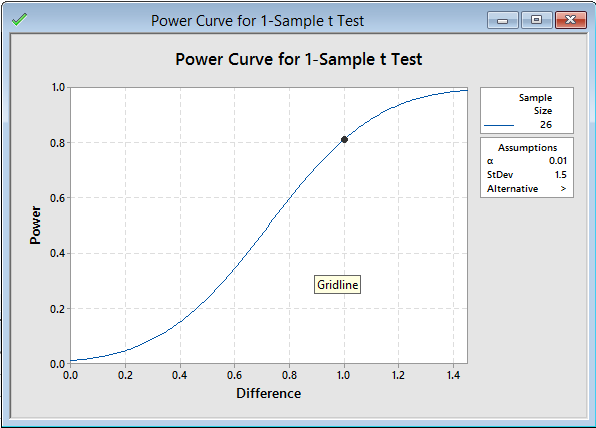
\includegraphics{./images/powercurve.png}
 % powercurve.png: 596x428 pixel, 96dpi, 15.77x11.32 cm, bb=0 0 447 321
\end{figure}


We need to sample 26 bottles of detergent so that we can test the claim
with 80\% power at 1\% level of significance.


    % Add a bibliography block to the postdoc
    
    
    
    \end{document}
